\section{関連}
飛行支援システムの比較的整っている例としてDJI Phantom4Proでは以下のような支援システムが搭載されている
\begin{itemize}
  \item ビジョンシステム
  \begin{itemize}
    \item 前方,後方,下方ビジョンシステム 
    \item 動作範囲 0.7~30m 
    \item 映像の動きから自身の移動を検知したり,障害物検知を行う.
  \end{itemize}
  \item 赤外線検知システム
  \begin{itemize}
    \item 動作範囲 0.2~7m
    \item 障害物との距離を精密に計測する.
  \end{itemize}
\end{itemize}

一方でトイドローンの例として同じDJI製ドローンとしてTelloでは以下のような支援システムがある
\begin{itemize}
  \item ビジョンシステム
  \begin{itemize}
    \item 下方ビジョンシステム 
    \item 映像の動きから自身の移動を検知をする.
  \end{itemize}
  \item 赤外線検知システム
  \begin{itemize}
    \item 機体下方
    \item 床面との距離を計測する.
  \end{itemize}
\end{itemize}




他に運転支援ではなく,自動運転の例として以下のような研究がある.
本研究は運転支援から,簡易的な自動運転,次に完全な自動運転を目指しており自動運転や姿勢推定などについても関連研究として調査している.
基本的にドローンが自律飛行を行う際に必要とされる処理がいくつかある.そのうちの2つが自己位置推定と姿勢推定である.
自己位置推定とは,ドローンが飛行している空間の中で自分がどの位置にいるのかを認識する事である.姿勢推定とは自分が水平方向に対してどの程度傾いているのか,鉛直方向に対してどの程度回転しているかを認識することある.

これらを行なっている関連研究としてNanomap\cite{Nanomap}という飛行モデルがある.においては2D-LIDARを用いた飛行経路探索手法が取られており,取得した点群データを過去数フレーム分を記憶しておき,過去の数フレーム分のデータと現在のフレームとの点群の変量によっておおよその障害物の位置を認識している.こちらの手法では,物体を正確に捉えることは放棄し,不確実な部分を物体の存在している可能性のある範囲として捉えている.視野にある物体のある可能性も含めて1番物体が少ない方向を飛行経路として選定し,飛行している.

他に,ドローンに限らずロボット工学全般で利用されてきたOctomap\cite{Octomap}がある.
こちらもNanomapと同様にLIDARを用いて周辺の環境情報を扱うものであるが,こちらはLIDARを用いて実際に周囲を点群からモデリングして周辺状況を把握する.

Octomapではモデリングする際に近い点群同士を同じ物体としてまとめ1つのブロックにするということを繰り返し,樹構造的にブロックを生成する為,生成後のデータは繰り返す回数等のパラメータによっては小さく圧縮することもできる.
\begin{figure}[htbp]
  \begin{center}
    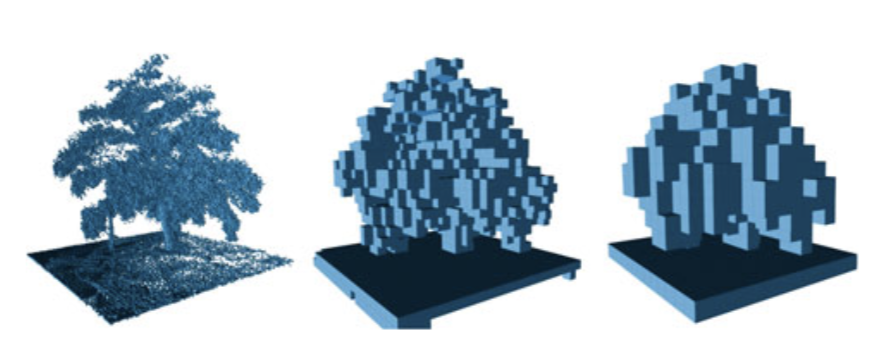
\includegraphics[clip,width=7.0cm]{img/octomap.png}
    \caption{圧縮率の違いによる生成物の違い}
    \label{fig:hamu}
  \end{center}
\end{figure}
しかし,実際に点群からモデルを生成するとなるとその計算量は非常に多く,高性能な小型コンピュータが現れている現在においても処理負荷が大きく,特にドローンにおいては積載量に制限がかかりやすい為扱いにくいものとなっている.


また,これらのようにLIDARを使用せず,CMOSセンサーのみで自律飛行を行なっている例もある.

実用性を備えた手のひらサイズ・完全オンボード処理 UAV のための 3 次元自己位置推定手法の提案と全自動飛行の実現\cite{SfMDrone}では自己位置推定で使用するセンサーはCMOSセンサーを利用した自律飛行を実現している.
CMOSセンサーからの映像をFPGAにストリームしてFAST\cite{FAST}による特徴点抽出処理を行い,その結果をBrief\cite{Brief}を用いて表現し,MCUに流し込み処理している.この研究での目的は外部処理系に依存せず,ドローン上で全て完結する自律飛行可能な小型ドローンの開発で,限定条件下(新聞紙を敷き詰めた床面)の上で飛行させ,特徴点を十分に検出できるようにした上で,飛行させ想定通りの飛行を実現している.

他に今回の研究のベース物としてDeepDrone\cite{DeepDrone}が挙げられる.こちらではドローンレースを自律飛行で行う為に自律飛行モデルを提案している.ドローンレースとは基本的にゲートを順に潜りながら飛行することが条件となっているドローン競技である.このゲートをRGBカメラで撮影した映像を推定モデルに対し,200*300の画像を所与として$\lbrace \vec{x}, v \rbrace$,を推定結果として得る.$\lbrace \vec{x}$は$\vec{x} \in [-1,1]^2$と定義され正規化された入力画像の中にある目標とするゲートへの方向を表していおり, $v \in [0,1]$ は飛行速度を正規化して表している.

DeepDroneでは訓練にシミュレータでのデータと現実世界でのデータを使っている.両者とも理想とする軌道とのズレを計算しそのズレを損失関数に入力し学習を進めていく.
\begin{figure}[htbp]
  \begin{center}
    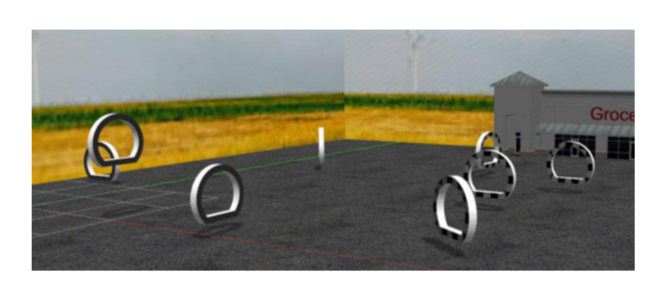
\includegraphics[clip,width=7.0cm]{img/deep-simu.png}
    \caption{シミュレータ上のゲート}
    \label{fig:gate}
  \end{center}
\end{figure}
シミュレータ上では直接理想とする軌道とのズレを取得し,実空間では実際に手動で実際のコース上を運び,ゲートを通過させるなどしてデータを収集していた.


他領域では自動運転という繋がりで自動運転車においても同様の回避システムは利用されており,これらから得られる物も多く,Honda\cite{Honda} では前方の安全運転支援システムだけでも以下のような物が挙げられる.

\begin{itemize}
\item 回避支援
  \begin{itemize}
    \item CMBS(衝突被害軽減ブレーキ)
    \item 誤発進抑制機能
    \item 路外逸脱抑制機能
    \item 歩行者事故軽減ステアリング
  \end{itemize}
\item 未然防止
  \begin{itemize}
    \item 渋滞追従機能(アダプティブクルーズコントロール)
    \item LKAS(車線維持支援システム)
    \item 先行車発進お知らせ機能
    \item 標識認識機能
  \end{itemize}
\end{itemize}
